% !TeX root = ../main.tex

% =================== 文獻探討 =================== %
\section{文獻探討}
本章旨在探討 5G-Advanced 網路能效優化之技術文獻。首先，依據 3GPP TR 38.864 技術報告確立網路節能（Network Energy Saving, NES）之範疇與四維度分類框架。接著，針對各維度之技術特徵與研究現況進行歸納比較，並進一步深入剖析空間域適應（Spatial Domain Adaptation, SDA）之現有文獻缺口。最後，本章將介紹李雅普諾夫最佳化（Lyapunov Optimization）理論，闡述其作為動態資源調度與穩定性控制之理論依據，為本研究之決策引擎建立理論基石。
\subsection{網路能源節省技術概論}
隨著 5G-Advanced 網路部署密度與天線陣列規模的指數級增長，行動網路能耗問題已成為電信營運商降低營運成本（OPEX）與達成淨零碳排目標之首要挑戰。為系統性應對此一挑戰，3GPP 於 Release 18 正式確立了 TR 38.864 技術報告 \cite{3gpp2023_tr38864}，專門針對新無線電（NR）系統的網路節能（NES）技術進行深度研究與標準化。該報告明確定義了基地台功耗模型，並將 NES 技術歸納為四個主要維度：時域（Time Domain）、頻域（Frequency Domain）、功率域（Power Domain）以及空間域（Spatial Domain）。

本研究對上述四維度技術之定義與潛能分析彙整如下：
\begin{itemize}[leftmargin=2em]
    \item \textbf{時域節能（Time Domain NES）：} 利用無線傳輸的不連續特性，透過 Cell DTX/DRX 機制，於數據空閒期間關閉部分射頻組件。
    \item \textbf{頻域節能（Frequency Domain NES）：} 根據業務負載量，動態調整操作頻寬部分（BWP）或調整載波聚合之啟用狀態，以降低頻譜處理能耗。
    \item \textbf{功率域節能（Power Domain NES）：} 透過動態調節基地台下行鏈路（DL）之功率放大器（PA）輸出功率，在確保覆蓋率前提下削減運作功耗。
    \item \textbf{空間域節能（Spatial Domain NES）：} 即空間域適應（SDA）技術，藉由 Massive MIMO 天線配置，在低負載時靜默冗餘的天線元件，實現能耗與系統負載的脫鉤。
\end{itemize}

\subsection{網路節能技術文獻探討 (四大領域)}
\subsubsection{時域節能（Time Domain NES）}
    時域節能技術之運作，建立於微秒級不連續傳輸（Micro-Discontinuous Transmission, uDTX）與先進休眠模式（Advanced Sleep Mode, ASM）之技術基礎上。uDTX 機制賦予基地台在微秒（$\mu s$）時間尺度內快速切換收發狀態的能力，並藉由 ASM 進入低功耗狀態以削減閒置能耗。在此技術基石下，目前 3GPP 研議之時域節能策略主要包含：週期性訊號適應（Periodic Signal Adaptation）、SSB-less 載波聚合（SSB-less Carrier Aggregation, SSB-less CA）、以及細胞不連續傳輸與接收（Cell Discontinuous Transmission/Reception, Cell DTX/DRX）等機制。

    透過動態調整同步訊號區塊（SSB）與系統資訊區塊 1（SIB1）之傳輸週期，或利用 Cell DTX/DRX 將用戶數據傳輸集中於特定時間窗，基地台得以創造更長之靜默期（Sleep Window），從而最大化 ASM 之啟用效益。如圖 \ref{fig:cell_dtx_drx} 所示，該機制透過對齊基地台的數據傳輸窗與用戶端的休眠週期，實現了跨層級的資源節能與同步排程。Nokia \cite{nokia2024_energy} 指出，透過此類時域資源的精細化調控，基地台能在維持覆蓋率與服務品質的同時，顯著降低非活躍時段的基礎能耗。

    \begin{figure}[htbp]
        \centering
        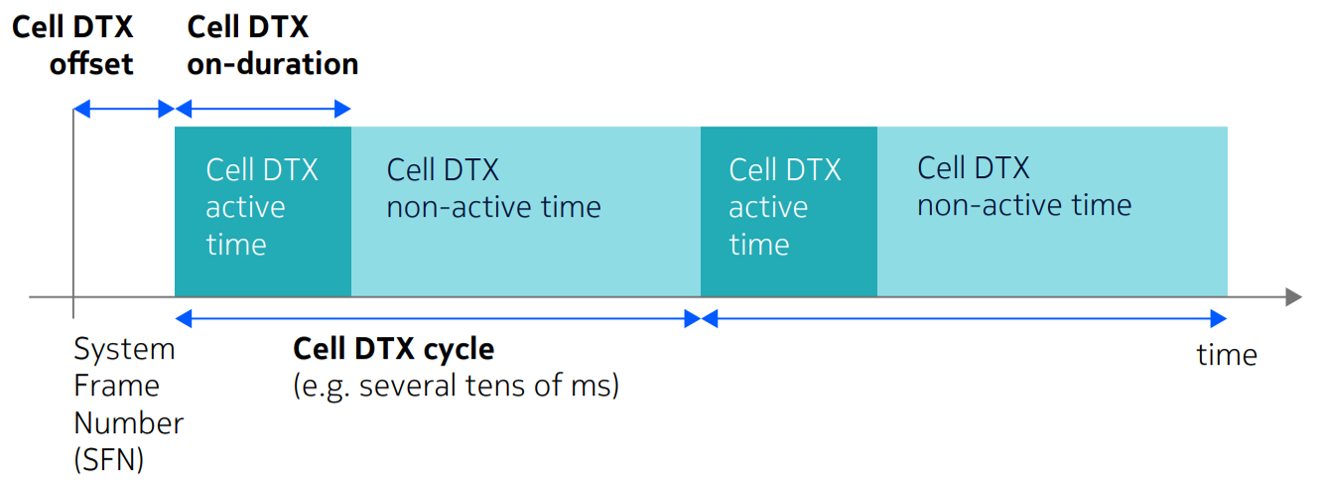
\includegraphics[width=0.9\textwidth]{figures/Cell DTXDRX示意圖.png} % 請確認您的檔名與路徑
        \caption{Cell DTX/DRX 運作示意圖（引自 \cite{nokia2024_energy}）}
        \label{fig:cell_dtx_drx}
    \end{figure}

    在產業標準與效能評估方面，Ericsson \cite{ericsson2022_r1_2212154} 針對 5G-Advanced 基地台定義了一套標準化的系統級模擬評估方法論，該研究深入量化了各種時域節能機制的功耗削減增益，並確立了時域資源調度在低負載場景下的效能與節能權衡基準。為了提升時域節能機制對於動態流量的適應性，近期學術界轉向探討智慧化控制策略。例如，Mao et al. \cite{mao2023_drl} 提出以深度強化學習（DRL）為基礎的 Cell DTX/DRX 設定策略，透過數據驅動的方式動態調整休眠參數，克服了傳統靜態配置無法因應網路突發流量的侷限，標誌著當前時域節能技術由「規則驅動」邁向「智慧感知」之研究進程。
\subsubsection{頻域節能（Frequency Domain NES）}
    頻域節能技術的核心思維在於透過動態調整頻譜資源之使用，以降低基地台的處理能耗。此類技術主要包含頻寬部分調適（Bandwidth Part, BWP Adaptation）以及載波聚合（Carrier Aggregation, CA）策略。其機制係依據當前網路負載狀況，動態限制基地台處理之頻率資源範圍，或關閉部分頻段之操作，藉此減少基頻處理單元（Baseband Processing Unit）與相關射頻鏈路之運作負荷。
    
    然而，根據 Oikonomakou et al. 之研究評估，在 3GPP TR 38.864 之系統級評估框架下，頻域節能技術雖具備調整彈性，但與時域或空間域節能技術相比，其整體的網路節能增益（NES gain）潛力表現相對有限。該研究指出，頻域節能策略在 3GPP 對於 5G-Advanced 基地台的研究中，多被視為優先級較低之選項，主要原因在於其節能增益潛力不如其他技術維度顯著\cite{oikonomakou2023_power}。
    
    此外，頻域節能技術亦面臨與服務品質（QoS）維護的權衡挑戰。頻寬的縮減將直接影響終端設備之使用者體驗吞吐量（User-Perceived Throughput, UPT），在網路負載變動頻繁的場景下，過度頻繁的頻譜調整不僅難以帶來顯著能耗削減，反而可能因為頻寬切換與參數重新配置，增加系統信令負擔並降低整體頻譜使用效率。因此，在當前 5G 網路能源節省技術的發展路徑中，頻域調適技術多作為輔助性策略，而非核心之節能引擎。
\subsubsection{功率域節能（Power Domain NES）}
    功率域節能技術之核心機制在於動態調整下行鏈路（DL）訊號與實體通道（例如實體下行分享通道，PDSCH）的發射功率。在傳統 5G NR 標準規範中，基地台主要依賴半靜態（Semi-static）配置之功率偏移參數（如 \texttt{powerControlOffset}）來決定資料通道相對於參考訊號（如 CSI-RS）之發射功率。文獻指出，為了避免影響處於覆蓋邊緣的傳統使用者設備，此技術應優先應用於使用者專屬通道（UE-dedicated channels），而避免對全區廣播訊號（如 SSB）進行降功率處理 \cite{3gpp2023_tr38864}   
    在節能潛力與系統效能的評估上，Oikonomakou et al. \cite{oikonomakou2023_power} 針對 5G-Advanced 基地台進行了深度的系統級模擬與探討。評估結果顯示，若將基地台的發射功率靜態調降 3dB、6dB 與 9dB，依據網路負載的不同，約可帶來 3\% 至 20\% 的網路節能增益（NES gain）。其中，在輕度與中度負載場景下，由於調降功率的比例較高，此類策略能反映出相對較佳的節能效果。

    然而，功率域節能技術伴隨著嚴峻的效能妥協。發射功率的降低會直接導致接收端之訊號干擾雜訊比（SINR）惡化，進而對使用者體驗吞吐量（UPT）造成顯著的負面衝擊。該研究數據表明，即使僅調降 3dB，仍會造成高達 12\% 的 UPT 損失；若採取更為激進的 6dB 或 9dB 降幅，UPT 的損失幅度甚至會急遽擴大至 6\% 至 33\% \cite{oikonomakou2023_power}。

    綜上所述，功率域節能技術雖然提供了直觀的降功耗手段，但其所能取得的節能增益（最高 20\%）與其對系統傳輸速率的破壞性（高達 33\% 損失）呈現極大的不對等。加上現有半靜態參數配置缺乏對動態突發流量的即時適應能力，導致服務品質（QoS）難以獲得有效保障。基於上述效能瓶頸，在 3GPP 針對 5G-Advanced 節能機制的研議中，純粹的功率域調降技術已被列為較低優先級（de-prioritized）之選項。

\subsubsection{空間域節能（Spatial Domain NES）}
空間域適應（Spatial Domain Adaptation, SDA）技術係透過 Massive MIMO 天線陣列之高度自由度，針對基地台之實體天線單元（Antenna Elements）或收發鏈路（TXRU）進行動態關斷（Muting），以實現能耗與系統負載的解耦。在 5G-Advanced 的節能架構中，SDA 被視為最具能源效益潛力之手段。

根據 3GPP TSG-RAN WG1 Meeting \#112 的相關技術討論 \cite{huawei2023_r1_2302179}，針對空間域適應的硬體映射架構，業界主要歸納為三種常見的實作類型（如圖 \ref{fig:sda_types} 所示）：
\begin{itemize}
    \item \textbf{Type 1 (Subarray-1):} 所有關聯於單一邏輯天線埠之空間元素被視為一個群組，進行整體性的啟用或關閉。
    \item \textbf{Type 2 (Subarray-2):} 僅針對關聯於邏輯天線埠之空間元素子集進行啟用或關閉，提供較為細緻的能耗控制。
    \item \textbf{Type 3 (Full-connection):} 採用全連接架構，TxRU 與天線陣列間存在更為靈活的映射矩陣，允許在維持邏輯埠定義的前提下，動態調整硬體鏈路與天線元件之連接關係，藉此在關閉部分資源之餘維持較佳的波束成形效能。
\end{itemize}

\begin{figure}[htbp]
    \centering
    
\includegraphics[width=1\textwidth]{天線域適應作法.png}
    \caption{3GPP TR 38.864 空間域適應之天線調整方式分類（引自 \cite{huawei2023_r1_2302179}）}
    \label{fig:sda_types}
\end{figure}

在技術性能評估方面，vivo 於 3GPP 之技術貢獻 \cite{vivo2022_r1_2212541} 深入分析了 SDA 之節能潛力。該研究透過對比「半靜態（Semi-static）」與「動態（Dynamic）」天線調整策略，證實了基於瞬時負載（Instantaneous Load）的即時調整機制，能夠在輕載時最大化能耗削減，並在高負載尖峰時刻迅速恢復系統容量，進一步突顯了動態演算法對於 SDA 應用場景之必要性，而非僅依賴固定的時間排程。

為進一步突破單一技術維度之節能瓶頸，近年研究開始聚焦於空間域與功率域之聯合調適，試圖透過跨層策略克服單純天線靜默帶來的效能損失。

Ribeiro et al. \cite{ribeiro2024_power} 針對天線縮減（Antenna Reduction）所引發的物理層副作用進行了深入探討。該研究指出，當基地台減少天線陣列（Antenna Array）的作動數量時，波束寬度（Beamwidth）會隨之增加。此種「波束變寬（Beam Broadening）」現象不僅降低了空間解析度，更會顯著增加鄰區間的訊號洩漏與干擾（Inter-cell Interference），進而惡化系統邊緣使用者的 SINR。為解決此一難題，該研究提出了一種自適應設計，在執行天線靜默的同時，引入功率提升（Power Boosting）策略。透過精準控制剩餘天線的發射功率，該機制在維持既有覆蓋範圍與訊號強度的前提下，成功緩解了因波束變寬而惡化的干擾問題，實現了節能與連線品質的平衡。

另一方面，Ravi et al. \cite{ravi2026_energy} 則將此概念擴展至更具彈性的「動態聯合調適（Dynamic Joint Adaptation）」框架。不同於前述研究較靜態的補償機制，該文提出了一種基於瞬時負載的聯合優化演算法，將天線配置數量與發射功率視為一組耦合的決策變數。其做法是根據每一調度週期（Scheduling Cycle）的網路負載變化，動態計算最佳的天線埠組合（Antenna Subset）與對應之發射功率分配。實驗數據證實，這種閉環的聯合優化方法，不僅能比傳統單維度節能策略獲得更高的整體能源效率（Energy Efficiency, EE），更具備了針對突發流量（Burst Traffic）進行快速資源重組的能力。

此外，SDA 技術在實作面上亦需考量相關的技術挑戰。當基地台動態調整天線配置時，終端設備（UE）需因應天線模式的變更進行通道狀態資訊（CSI）的量測與回報，若缺乏有效的管理機制，可能導致控制平面的信令開銷增加。針對此一議題，學界已有相關探討，例如 Wang 等人 \cite{wang2025_csi} 提出基於巢狀碼本（Nested Codebook）的 CSI 回報架構，透過優化碼本結構以降低頻繁天線切換所引發的回報負擔。此類研究反映了 SDA 在邁向實務部署時，對於降低 CSI 回報信令開銷之技術需求，是該領域目前持續探討的實務課題。

綜上所述，儘管 SDA 技術在提升能效上展現出巨大潛力，但現有文獻多聚焦於特定架構下的開路評估或靜態閾值策略。面對真實網路中高度隨機的突發流量（Burst Traffic），傳統方案難以在『深度節能』與『嚴格的延遲保障（QoS）』之間取得即時且動態的平衡，極易導致天線配置震盪與佇列延遲的非預期發散。現有方案顯然缺乏一套具備流量感知能力、且能在硬體開銷與系統穩定性間精準調度的閉環控制機制。



\subsection{李雅普諾夫最佳化理論於無線網路之應用 (Lyapunov Optimization)}
李雅普諾夫最佳化（Lyapunov Optimization）作為一種處理隨機系統穩定性與效能權衡的數學工具，已被廣泛應用於無線通訊網路的資源排程與管理 \cite{neely2006energy, neely2010_stochastic}。該理論的核心價值在於提供了一套無需預測未來流量統計特性的線上決策（Online decision making）框架，使系統僅需依賴當前時槽的狀態，即可在滿足網路佇列穩定性的前提下，達成長期時間平均效能的最佳化，從而規避了傳統隨機規劃（Stochastic Programming）中對未來流量分佈精確估計的依賴。

在理論發展脈絡上，Neely \cite{neely2006energy} 首先確立了漂移加懲罰（Drift-Plus-Penalty）的優化框架，透過數學證明釐清了無線網路中「傳輸功耗」與「佇列延遲」之間不可分割的權衡關係，並定義了系統效能收斂的理論邊界。隨後，Neely \cite{neely2010_stochastic} 進一步將該方法論系統化，發展出涵蓋多跳傳輸、能量採集等多維度資源調度的通用工程架構，而 Neely \cite{neely2012_lyapunov} 則針對排隊網路的穩定性進行了深度分析，證實該演算法在強收斂準則下，即便面對突發性流量與高動態環境，仍能確保網路佇列的強健穩定性。

\subsubsection{網路排程演算法之比較與核心優勢}
在面對通訊網路之動態資源配置與空間域適應（SDA）時，傳統演算法通常面臨不同程度之侷限性。為了突顯本研究採用李雅普諾夫最佳化之合理性與必然性，以下針對常見之三類決策演算法進行對比：

\begin{itemize}
    \item \textbf{啟發式演算法（Heuristic Algorithms）}：如基於資源利用率閾值之天線切換機制。此類方法實作簡易且運算複雜度極低，然其本質屬「被動觸發（Passive-triggered）」控制。系統僅於負載越過硬性閾值後方遲滯地執行天線切換，缺乏嚴謹之數學邊界保證。面對 5G 網路高度非平穩之突發流量（Bursty Traffic）時，僵化之閾值判定極易導致基地台於相鄰時槽間頻繁啟閉天線，進而引發嚴重之信令乒乓效應（Ping-pong Effect）。此外，該類方法多仰賴經驗法則設定參數，無法於數學層面精確定量「能效提升」與「延遲折損」間之權衡關係。
    
    \item \textbf{傳統最佳化理論（Traditional Optimization）}：如動態規劃（Dynamic Programming）或非線性規劃（Non-linear Programming）。於通訊排程場景中，實體層傳輸速率與天線配置呈高度非線性關係（如 Shannon 容量受多重干擾與多徑衰落影響），難以簡化為低複雜度之線性模型。此外，為求得長期時間跨度下之全局最佳解（Global Optimum），此類演算法通常要求預先掌握未來所有時間點之「通道狀態資訊（CSI）」與「封包到達率」（即 A priori knowledge）。於毫秒級動態變化之 5G 通道環境中，此種高度依賴未來資訊之非因果（Non-causal）假設，在工程實務上並不具可行性。
    
    \item \textbf{馬可夫決策過程與強化學習（MDP \& Reinforcement Learning）}：此類演算法雖具備強大之環境學習能力，然於實務部署上面臨嚴峻挑戰。傳統 MDP 面對具備高度連續性特徵之佇列積壓狀態時，極易因狀態與動作空間之擴張，導致轉移矩陣呈指數級膨脹，進而陷入「維度災難（Curse of Dimensionality）」。而近年廣受矚目之深度強化學習（Deep RL）雖可透過神經網路取代查表以緩解維度問題，然其應用於 5G MAC 層（如 TTI = 0.5 毫秒）時仍具三大瓶頸：其一為分佈偏移與黑箱風險，離線訓練之模型面對真實場景之突發流量時，極易因分佈偏移（Distribution Shift）產生不可預期之決策失誤；其二為硬體能耗開銷，毫秒級之頻繁神經網路推論將衍生龐大之運算能耗，抵銷 SDA 機制之節能初衷；其三為缺乏數學邊界保證，該類演算法難以為系統最壞情況（Worst-case）之佇列穩定性提供嚴謹之理論保障。
\end{itemize}

相較之下，李雅普諾夫最佳化理論完美克服了上述演算法的痛點。其最大特性在於\textbf{「無需預知未來（Requires no future knowledge）」}。它僅依賴當前時槽的即時觀測值（如當前佇列長度與通道狀態）即可進行決策，並能在數學上嚴格證明演算法具備 $\mathcal{O}(V)$ 的佇列延遲邊界，以及逼近理論最佳值 $\mathcal{O}(1/V)$ 的能耗表現。這種極低運算複雜度且具備理論保證的「線上決策（Online Decision）」特性，使其成為本研究 SDA 決策引擎之首選。

\subsubsection{現有文獻於通訊資源分配之應用探討}
隨著通訊系統日益複雜，李雅普諾夫最佳化架構亦被廣泛延伸至各類複雜的無線通訊場景。在行動邊緣運算（MEC）領域，Mao 等人 \cite{mao2016_power_delay} 提出基於該理論的任務卸載與資源配置策略，證實系統能透過動態調整運算資源與傳輸功率，在確保任務佇列穩定且不壅塞的前提下，靈活地在「設備功耗」與「執行延遲」之間取得平衡。

此外，Kim 與 Choi \cite{kim2021_lyapunov_uav} 亦將此框架推廣至無人機（UAV）通訊網路，設計出高能效的多路徑資料傳輸策略。該研究透過「漂移加懲罰」方法，在動態網路拓撲與不確定的流量負載下，動態決策封包傳輸路徑與功率分配。此方法不僅成功解決了因路徑多樣性（Path diversity）而衍生的能耗增長問題，更在維持無人機傳輸穩定性與資料延遲容忍度（Delay-tolerant）的條件下，顯著優化了整體的傳輸效率。

\subsubsection{傳統固定權重控制之侷限性}
儘管上述文獻 \cite{mao2016_power_delay}\cite{kim2021_lyapunov_uav} 成功利用李雅普諾夫理論解決了多目標權衡問題，但其決策架構大多採用「固定的控制權重（Fixed $V$）」。在真實 5G 基地台的場景中，網路流量通常呈現高度非平穩（Non-stationary）與突發性（Bursty）特徵。若採用固定的 $V$ 值，系統將無法適應動態的負載變化：當 $V$ 值設定過大時，基地台在突發流量下容易導致佇列崩潰；若設定過小，則在輕載時無法徹底釋放硬體休眠之節能潛力。此一傳統框架之盲點，突顯了發展「動態流量感知（Traffic-Aware）」機制的迫切需求，此即為本研究第三章所欲解決之核心問題。

\subsection{研究缺口與動機總結}
綜合前述文獻探討，為因應 5G-Advanced 網路持續攀升的營運能耗，3GPP TR 38.864 確立了四大網路節能（NES）維度 \cite{3gpp2023_tr38864}。其中，空間域適應（SDA）技術憑藉其直接關閉實體天線單元與射頻鏈路的能力，展現了最為顯著的硬體節能潛力。然而，如何在維持使用者服務品質（QoS）的前提下，最大化 SDA 的節能效益，仍是當前產業界與學術界亟需解決的難題。
歸納現有針對 SDA 的文獻與標準提案，主要受限於以下三大研究缺口：
\begin{enumerate}
    \item \textbf{無法有效適應突發流量：} 傳統基於固定負載門檻值（Load-based）或半靜態（Semi-static）的決策機制，在面對 5G 真實環境中高度隨機的突發流量（Burst Traffic）時，往往反應遲鈍或過度敏感。
    \item \textbf{乒乓效應與延遲發散：} 缺乏完善防呆機制的天線頻繁收放，極易引發「乒乓效應（Ping-Pong Effect）」。這不僅徒增系統信令與硬體切換的負擔，更會導致 MAC 層封包佇列（Queue）急遽累積，引發難以收斂的傳輸延遲。
    \item \textbf{缺乏跨層聯合優化（Cross-layer Optimization）機制：} 現有研究多數僅停留在單一實體層（PHY）的開路評估，缺乏將 MAC 層排程延遲與 PHY 層整體功耗進行跨層閉環控制的嚴謹演算法。
\end{enumerate}

基於上述痛點，本研究之核心動機在於引進並「改良」具備嚴謹數學基礎之李雅普諾夫最佳化（Lyapunov Optimization）理論。本研究突破了傳統靜態權重的侷限，創新提出具備「動態 $V$ 值調適（Dynamic $V$ Adaptation）」機制的決策引擎。透過「漂移加懲罰（Drift-Plus-Penalty）」框架與動態 $V$ 值的結合，系統能在突發流量湧入時瞬間調控權重以加速清空佇列（確保 QoS），並在流量平緩時切換權重以實現極致節能，完美克服了傳統機制無法兼顧的兩難。

總結而言，本論文致力於設計一套符合 3GPP 國際標準架構之「流量感知動態天線調適引擎」。本研究不僅將進行嚴謹的數學推導，更將深入修改並擴充 C++ 系統級模擬器。透過真實的大規模網路模擬，本論文將證明所提之動態李雅普諾夫決策機制能有效克服乒乓效應，在高度動態的 5G 網路環境中，實現網路能效（ESG）與服務品質的最佳化權衡。